\documentclass[12pt]{beamer}
\usetheme{Rochester}
\usepackage[utf8]{inputenc}
\usepackage{amsmath}
\usepackage{amsfonts}
\usepackage{amssymb}
\usepackage{amsthm}
\usepackage{graphicx}
\usepackage{cite}

\newtheorem{myDef}{Definition}

\author{Josiah Hanna, David Tamez, and Xiaorong Zhu}
\title{Generating Petri Nets With Evolutionary Algorithms}
\institute{The University of Texas at Austin}
\date{December 3rd, 2014}
\begin{document}

\begin{frame}
\titlepage
\end{frame}

\begin{frame}{Petri Net Overview}
High level definition of a Petri Net
\begin{myDef}
A Petri Net is defined as a tuple $(P,T,F,M,W)$ where $P$ is a set of place nodes, $T$ is a set of transition nodes, $F$ is a set of arcs in either $P \times T$ or $T \times P$, $M: P \rightarrow Z$ is an initial marking, and $W: F \rightarrow Z$ is an arc weight function.
\end{myDef}
\begin{figure}
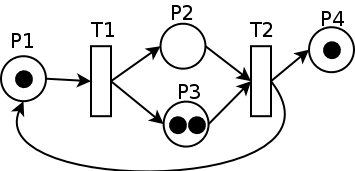
\includegraphics[scale=0.25]{petri_net}
\caption[]{An example Petri network \label{exampleNet}}
\end{figure}
\end{frame}

\begin{frame}{Petri Net Applications and Disadvantages}

Applications
\begin{itemize}
\item apply them
\end{itemize}
Disadvantages
\begin{itemize}
\item Symbolic approach
\item Must be hand coded which is hard for complex tasks
\end{itemize}

Solution: 

\centering{\Large{Use evolutionary algorithm to evolve them!}}

\end{frame}

\begin{frame}{Proposed Solution}

We propose that the Neuroevolution of Augmenting Topologies (NEAT) could be used to evolve Petri Nets

\begin{itemize}
\item NEAT evolves topologies and weights of neural networks.
\item NEAT allows complex structures to evolve through speciation.
\end{itemize}

\end{frame}

\begin{frame}{Genome}
Place Node Gene

Transition Node Gene

Link Gene

\end{frame}

\begin{frame}{Genetic Operators}

We use the following mutation operators in evolving our network:
\begin{itemize}
\item mutate add node
\item mutate add link
\item mutate node
\item mutate link
\end{itemize}

\end{frame}

\begin{frame}{Target Task}
We evolve Petri net solutions for a robot moving towards a goal in a grid world.
\begin{figure}
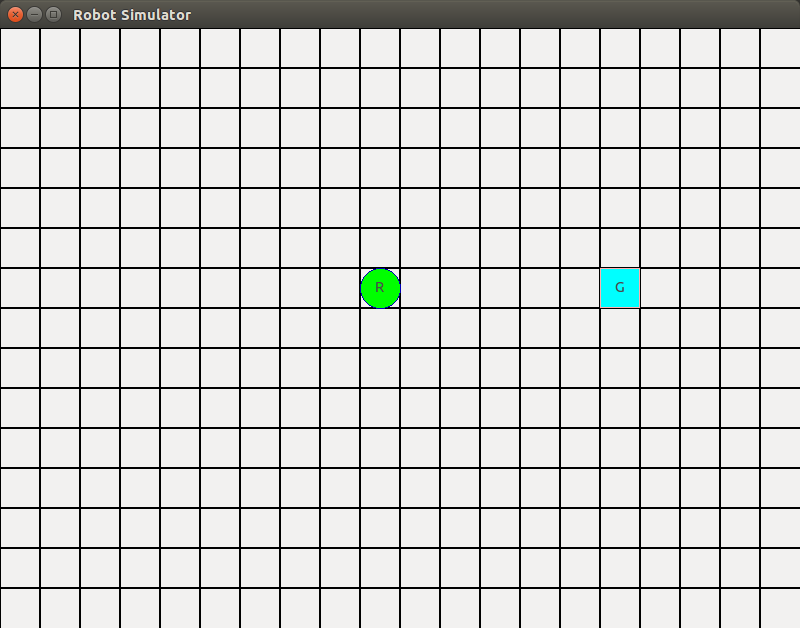
\includegraphics[trim = 80mm 80mm 20mm 70mm, clip, width = 2.4in, height = 1.6in]{robot_sim.png}
\end{figure}
We define the fitness of a potential solution to be:
$$fitness = \frac{startDistanceToGoal}{finalDistanceFromGoal + actionsTaken}$$
\end{frame}

\begin{frame}{Results}

\end{frame}

\begin{frame}{Resulting Structure}

\end{frame}

\begin{frame}{Future Work}
The next steps in exploring Petri net evolution are:
\begin{enumerate}
\item Add cross over operations to the evolutionary algorithm.
\item Explore different mutation operators.
\item Generate more complex types of Petri networks.
\item Increase the complexity of our target task.
\item Add methods to combine Petri nets into hierarchies.
\end{enumerate}

\end{frame}

\begin{frame}{References}

\end{frame}

\end{document}